\documentclass[UTF8]{resume}

\name{Licheng Zheng}
\address{\faPhone~+86 189 1892 8753 \faEnvelope~\href{mailto://zhenglicheng@shu.edu.cn}{zhenglicheng@shu.edu.cn} \faGithub~\href{https://github.com/SHUzheking/}{GitHub: SHUzheking} \faWeixin~2035451658~~~~~}
\address{}

\begin{document}

\begin{tikzpicture}[remember picture, overlay] 
    \node[anchor = north east] at ($(current page.north east)+(-1.3cm,-1.2cm)$) {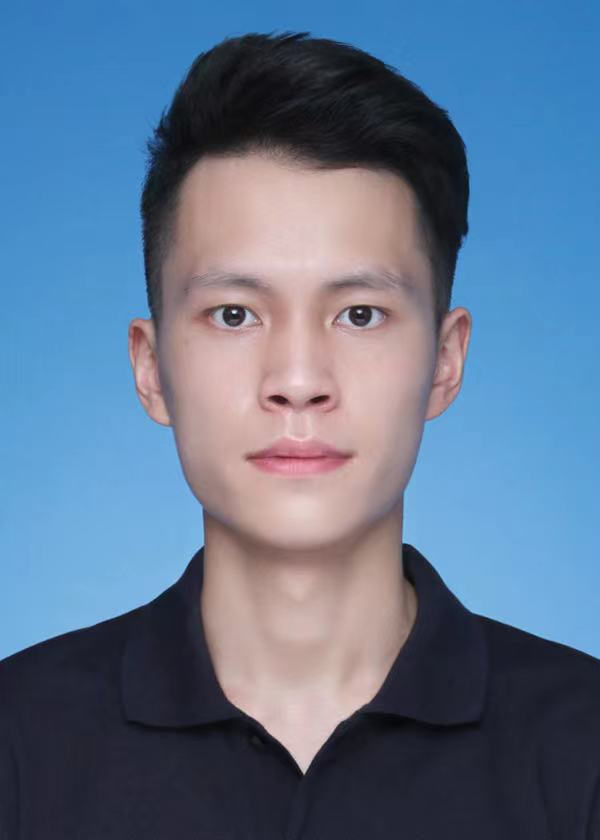
\includegraphics[height=2.5cm]{avatar.jpg}};
\end{tikzpicture}
  
\begin{rSection}{\faCogs~Skill Set}
    \begin{itemize}
        \itemsep -0.5em
        \item Familiar with C++, Python, HTML, CSS, MATLAB.
        \item Basic experience in Vue, JavaScript, Java, SQL, CUDA programming.
        \item Hands-on experience in Ubuntu and git on daily basis.
        \item Comprehend C-Compiling methods, machine learning, deep learning.
    \end{itemize} 
\end{rSection}

\begin{rSection}{\faGraduationCap~Education}
    %\begin{itemize}
    Shanghai~University\quad Artificial Intelligence major \quad GPA~84.7/100\hfill Sep 2021-Now\\
    %\end{itemize}
\end{rSection}
 

\begin{rSection}{\faUsers~Projects}

    \begin{rProject}{School Research}{Research on automatic descriptor acquisition method for NASICON electrolyte}{May 2022 - Mar 2023}
        \textbf{Overview}: Using the text mining method, descriptors can be extracted from small batch of NASICON solid electrolyte documents and trained based on this model to achieve automatic and efficient acquisition of NASICON solid electrolyte descriptors.\\
        \textbf{Content}: Using \textbf{Vue} to develop front-end interfaces and the back-end deployment using \textbf{Springboot} to communicate with \textbf{MySQL} and \textbf{Neo4j} databases. BERT algorithm are deployed using \textbf{Pytorch} for paper processing, and the extracted descriptors are used to construct the knowledge map using \textbf{Neo4j} database.
    \end{rProject}

    \begin{rProject}{Group Project}{Computer Vision Algorithm Recognition System for RoboMaster Robots}{Oct 2021 - Dec 2022}
        \textbf{Overview}: Through the video stream of industrial camera deployed on the robot, this project can identify enemy robots' armor plates, and publish the target coordinate information to lock the platform at the recognition center. Its performance is similar to a self-aiming plugin in First-person shooting games.\\
        \textbf{Content}: The Yolo network is deployed on \textbf{Ubuntu} using \textbf{CUDA}. Kalman filter and trajectory model are used to improve the impact point of the projectile and achieve accurate strike.
    \end{rProject}

\end{rSection}

\begin{rSection}{\faAward~Awards}
    \begin{itemize}
        \itemsep -0.5em
        \item Third prize in The 21st National Undergraduate Robot Competition (RoboMaster 2022). \hfill Aug 2022
        \item First prize in The 35th Shanghai Youth Science and Technology Innovation Competition. \hfill Apr 2020
        \item First prize in Shanghai Youth Robot Knowledge and Practice Competition. \hfill Nov 2018, and Nov 2019
        \item First prize in Shanghai Youth AI Competition. \hfill Nov 2018
    \end{itemize}
\end{rSection}
\end{document}
